
\section{Shape of a dusty radiative bow wave}
\label{sec:shape-dust-wave}

As an alternative to hydrodynamic or magnetohydrodynamic bow shocks,
it is possible that some observed emission arcs may be bow waves due
to the action of radiation pressure on dust grains.

\begin{figure}
  \centering
  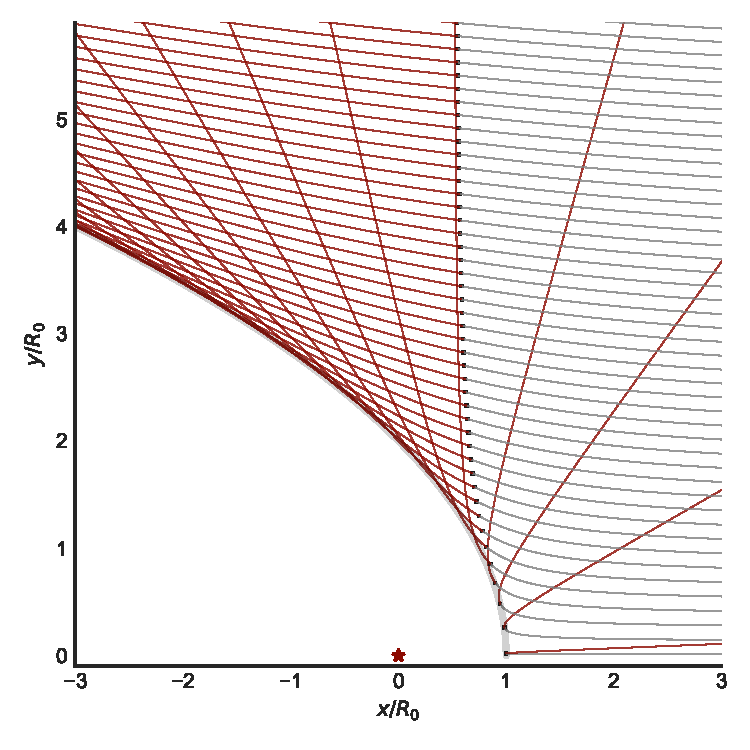
\includegraphics[width=\linewidth]{figs/dust-trajectories}
  \caption[Dust grain trajectories]{Dust grain trajectories under
    influence of a repulsive central \(r^{-2}\) radiative force.  Dust
    grains approach from the right at a uniform velocity and with a
    variety of impact parameters (initial \(y\)-coordinate). The
    central source is marked by a red star at the origin, and its
    radiative force deflects the trajectories into a hyperbolic shape,
    each of which reaches a minimum radius marked by a small black
    square.  The incoming hyperbolic trajectories are traced in gray
    and the outgoing trajectories are traced in red.  The locus of
    closest approach of the outgoing trajectories is parabolic in
    shape (traced by the thick, light gray line) and this constitutes
    the inner edge of the bow wave. }
  \label{fig:dust-trajectories}
\end{figure}

\begin{figure*}
  \centering
  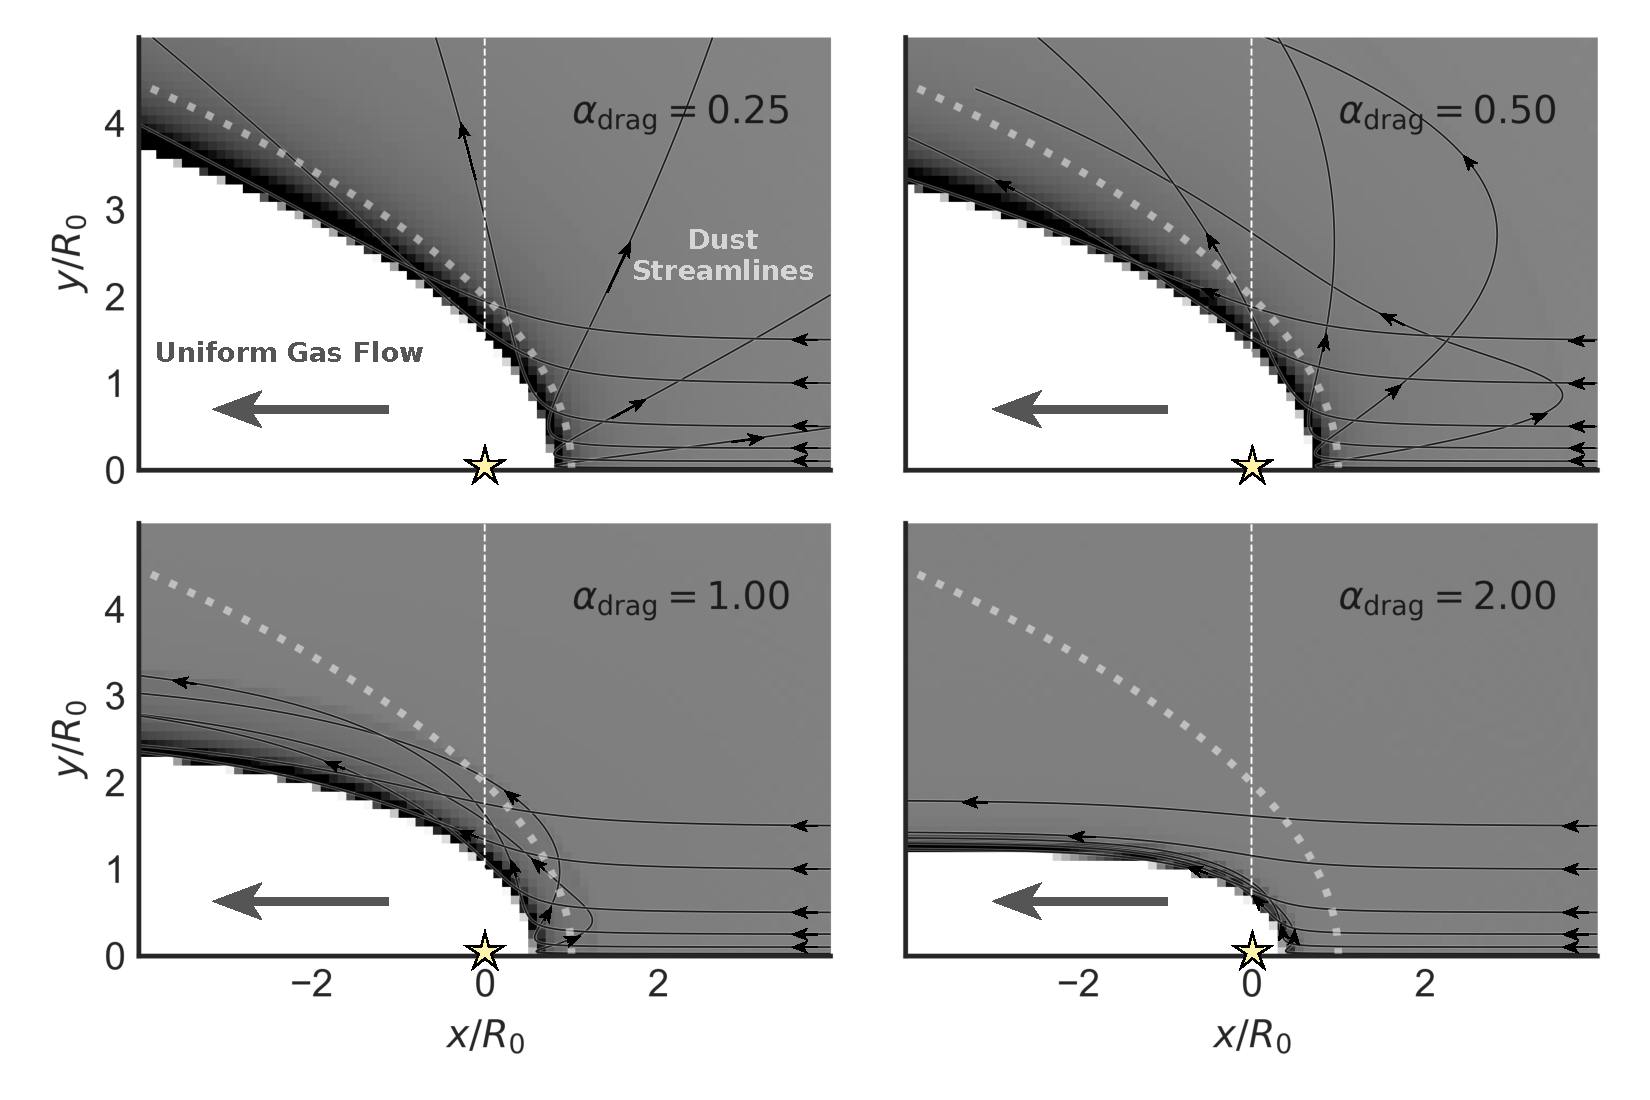
\includegraphics[width=\linewidth]{figs/dust-couple-stream-annotate}
  \caption{Dust grain trajectories under influence of gas drag in
    addition a repulsive central radiative force.  The dust
    streamlines are shown in blue and the dust density as a linear
    color scale, with maximum (white-yellow) of twice the ambient dust
    density.  Results are shown for four values of the drag parameter
    (see text): \(\alpha_\text{drag} = 0.25\), \(0.5\), \(1.0\), and
    \(2.0\). The shape of the bow wave for the drag-free case
    (Fig.~\ref{fig:dust-trajectories}) is shown by the thick dotted
    line.}
  \label{fig:dust-wave-coupling}
\end{figure*}

%%% Local Variables:
%%% mode: latex
%%% TeX-master: "quadrics-bowshock"
%%% End:
